Im Menü \enquote{Data-Input} (siehe \autoref{fig:instr_admin_absentees_dimenu}) können über den Auswahlpunkt \enquote{Fehlende eintragen}  fehlende Lehrer und fehlende Klassen eingegeben werden. Es öffnet sich ein weiteres Menü (siehe \autoref{fig:instr_admin_absentees_menu}) mit der Wahlmöglichkeit zwischen Lehrer und Klassen.
\begin{figure}[H]
\centering
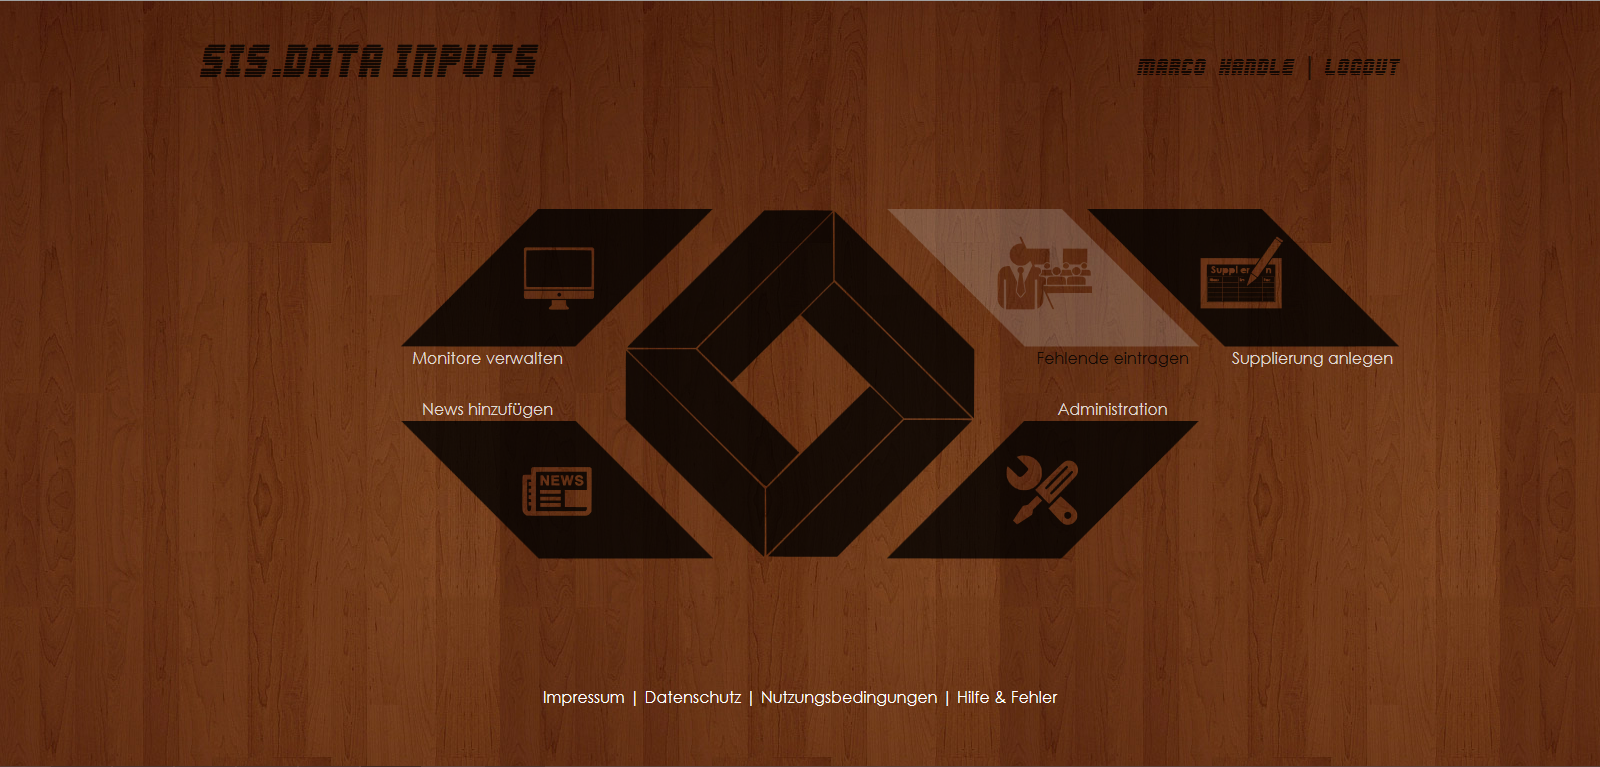
\includegraphics[keepaspectratio=true, width=14cm]{images/screenshots/data-inputs2.png}
\caption{Data-Input-Menü}
\label{fig:instr_admin_absentees_dimenu}
\end{figure}
\begin{figure}[H]
\centering
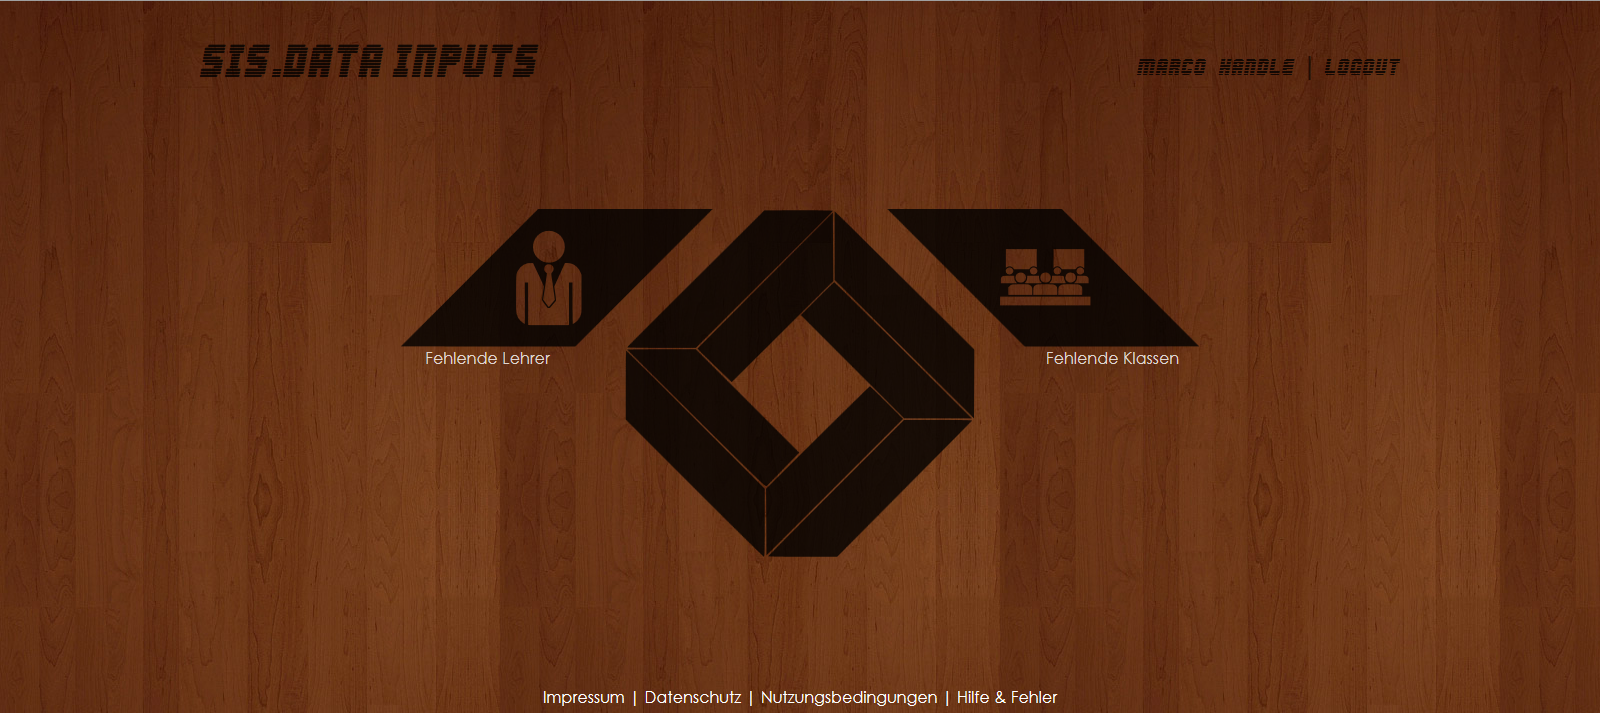
\includegraphics[keepaspectratio=true, width=14cm]{images/screenshots/data-inputs_absentees.png}
\caption{Fehlende Auswahl}
\label{fig:instr_admin_absentees_menu}
\end{figure}
\subsection{Fehlende Lehrer}
\label{sec:instr_admin_absentees_teacher}
In der tabellarischen Eingabemaske (siehe \autoref{fig:instr_admin_absentees_Lehrer}) können nun fehlende Lehrer hinzugefügt, Einträge geändert oder gelöscht werden. Standardmäßig werden beim Öffnen der Eingabemaske die für den aktuellen Tag erfassten Fehlenden Lehrer angezeigt.
\subsubsection{Fehlenden Lehrer Hinzufügen} \label{sec:instr_admin_absentees_teacher_insert}
Als erster Schritt ist das Datum des Tages auszuwählen, für den fehlende Lehrer erfasst werden. Dies kann entweder durch das Vor- und Zurückblättern mit den Pfeiltasten erfolgen oder durch eine manuelle Eingabe (Format yyyy-mm-dd). Die manuelle Eingabe ist mit der Enter-Taste zu bestätigen. Dieses Datum wird in neuen Eingabezeilen automatisch in das Feld Starttag eingetragen. Dann sind die einzelnen Eingabefelder zu befüllen.\\
\begin{table}
\centering
\begin{tabular}{p{3 cm}p{6 cm}p{5 cm}}
   \toprule
   \textbf{Eingabefeld} & \textbf{Typ} & \textbf{Wertebereich} \\
   \midrule
          \textbf{Lehrer} & Text \newline Kürzel des Lehrers -Auswahl aus Listenfeld & \\
          \hline
          \textbf{Starttag} & Datum \newline Wird automatisch eingetragen und kann nicht verändert werden &  \\
          \hline
          \textbf{Start-Stunde} & nummerisch & 1-16\\
          \hline
          \textbf{Endtag} & Datum \newline Standardmäßig wie Starttag ist auf gewünschtes Datum zu ändern & Größer oder gleich Starttag und kein Samstag oder Sonntag \\
          \hline
          \textbf{End-Stunde} & nummerisch & 1-16 \newline Wenn Starttag und Endtag gleich, dann größer als Start-Stunde\\
          \hline
          Grund & Text - optional \newline Freie Texteingabe für den Grund des Fehlens & \\
   \bottomrule
\end{tabular}
\caption{Eingabefelder Fehlende}
\end{table}
Sind alle Pflicht-Eingabefelder befüllt, wird durch Drücken auf Übernehmen die Eingabezeile übernommen, wobei vorher eine Plausibilitätsüberprüfung vorgenommen wird. Sollte eine Fehleingabe bemerkt werden, wird in einem Popup-Fenster (siehe \autoref{fig:instr_admin_absentees_fail}) das fehlerhafte Feld angezeigt. Die Eingabefelder werden gelöscht und müssen neu erfasst werden. Bei einer fehlerfreien Übernahme wird in der Eingabezeile die Checkbox Löschen und eine weitere Eingabezeile angezeigt.
\subsubsection{Eingabezeile verändern}
Ein bereits übernommener Eintrag kann noch nachträglich verändert werden. Die Änderungen sind in den Feldern vorzunehmen und dann wie unter \autoref{sec:instr_admin_absentees_teacher_insert} für jede Eingabezeile zu übernehmen.
\subsubsection{Eingabezeile löschen}
Das Löschen eines fehlenden Lehrers erfolgt über die Checkbox \enquote{Löschen} der entsprechenden Eingabezeile. Diese muss ausgewählt werden und dann mit Übernehmen bestätigt werden. Es erfolgt keine weitere Sicherheitsabfrage und der Eintrag ist \textbf{unwiderruflich} gelöscht (siehe \autoref{fig:instr_admin_absentees_Leherer_delete}).
\begin{figure}[H]
\centering
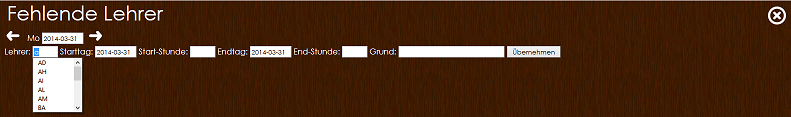
\includegraphics[keepaspectratio=true, width=16cm]{images/screenshots/absentees_teacher.png}
\caption{Fehlende Lehrer}
\label{fig:instr_admin_absentees_Lehrer}
\end{figure}
\begin{figure}[H]
\centering
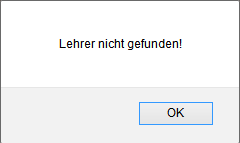
\includegraphics[keepaspectratio=true, width=4cm]{images/screenshots/input_fail_teacher.png}
\caption{Falsche Eingabe}
\label{fig:instr_admin_absentees_fail}
\end{figure}
\begin{figure}[H]
\centering

\includegraphics[keepaspectratio=true, width=16cm]{images/screenshots/absentees_teacher_delete.png}
\caption{Fehlenden Lehrer löschen}
\label{fig:instr_admin_absentees_Leherer_delete}
\end{figure}
\subsection{Fehlende Klassen}
Die Erfassung von Fehlenden Klassen erfolgt analog jener der Fehlenden Lehrer. Die Eingabemenüs und Eingabefelder sind sinngemäß wie unter \autoref{sec:instr_admin_absentees_teacher} beschrieben zu verwenden.